% A LaTeX (non-official) template for ISAE projects reports
% Copyright (C) 2014 Damien Roque
% Version: 0.2
% Author: Damien Roque <damien.roque_AT_isae.fr>

\documentclass{beamer}
\usepackage[utf8]{inputenc}
\usepackage[english]{babel}
\usepackage{palatino}
\usepackage{graphicx}
\graphicspath{{./images/}}
\usepackage{colortbl}
\usepackage{xcolor}
\usepackage{tikz}
\usetikzlibrary{shapes,arrows}
\usetikzlibrary{mindmap,trees}
\usetikzlibrary{calc}
\usepackage{pgfplots}
\pgfplotsset{compat=newest}
\pgfplotsset{plot coordinates/math parser=false}
\newlength\figureheight
\newlength\figurewidth
\usepackage{ifthen}
\usepackage{subfigure}
\usepackage{amsthm}
\usepackage{amsfonts}
\usepackage{amssymb}
\usepackage{amsmath}
\usepackage{eurosym}
\usepackage{wasysym}
\usepackage{tikz}
\usepackage{hyperref}
\usepackage{url}
\usepackage{epstopdf}
\usepackage{tkz-euclide}
\usepackage[font=small]{caption}
\usepackage{tkz-euclide}
\usepackage{animate}
\usetkzobj{all}
\DeclareCaptionFormat{person}{ #3 }
\epstopdfDeclareGraphicsRule{.gif}{png}{.png}{convert gif:#1 png:\OutputFile}
\AppendGraphicsExtensions{.gif}
% Printing on 2 slides per page
%\pgfpagesuselayout{2 on 1}[a4paper,border shrink=5mm]

% My macros...
\newcommand*{\SET}[1]  {\ensuremath{\boldsymbol{#1}}}
\newcommand*{\VEC}[1]  {\ensuremath{\boldsymbol{#1}}}
\newcommand*{\MAT}[1]  {\ensuremath{\boldsymbol{#1}}}
\newcommand*{\OP}[1]  {\ensuremath{\text{#1}}}
\newcommand*{\NORM}[1]  {\ensuremath{\left\|#1\right\|}}
\newcommand*{\DPR}[2]  {\ensuremath{\left \langle #1,#2 \right \rangle}}
\newcommand*{\calbf}[1]  {\ensuremath{\boldsymbol{\mathcal{#1}}}}
\newcommand*{\shift}[1]  {\ensuremath{\boldsymbol{#1}}}
\newcommand{\eqdef}{\stackrel{\mathrm{def}}{=}}
\newcommand{\argmax}{\operatornamewithlimits{argmax}}
\newcommand{\argmin}{\operatornamewithlimits{argmin}}
\newcommand{\ud}{\, \text{d}}
\newcommand{\vect}{\text{Vect}}
\newcommand{\sinc}{\text{sinc}}
\newcommand{\esp}{\ensuremath{\mathbb{E}}}
\newcommand{\hilbert}{\ensuremath{\mathcal{H}}}
\newcommand{\fourier}{\ensuremath{\mathcal{F}}}
\newcommand{\sgn}{\text{sgn}}
\newcommand{\intTT}{\int_{-T}^{T}}
\newcommand{\intT}{\int_{-\frac{T}{2}}^{\frac{T}{2}}}
\newcommand{\intinf}{\int_{-\infty}^{+\infty}}
\newcommand{\Sh}{\ensuremath{\boldsymbol{S}}}
\newcommand{\Cpx}{\ensuremath{\mathbb{C}}}
\newcommand{\R}{\ensuremath{\mathbb{R}}}
\newcommand{\Z}{\ensuremath{\mathbb{Z}}}
\newcommand{\N}{\ensuremath{\mathbb{N}}}
\newcommand{\K}{\ensuremath{\mathbb{K}}}
\newcommand{\reel}{\mathcal{R}}
\newcommand{\imag}{\mathcal{I}}
\newcommand{\cmnr}{c_{m,n}^\reel}
\newcommand{\cmni}{c_{m,n}^\imag}
\newcommand{\cnr}{c_{n}^\reel}
\newcommand{\cni}{c_{n}^\imag}
\newcommand{\LR}{\mathcal{L}_2(\R)}
\newcommand{\tproto}{g}
\newcommand{\rproto}{\check{g}}
\newcommand{\Tproto}{G}
\newcommand{\Rproto}{\check{G}}

%\theoremstyle{definition}
%\newtheorem{definition}{Définition}[subsection]

\theoremstyle{remark}
\newtheorem{remarque}{Remarque}[subsection]

\theoremstyle{plain}
\newtheorem{propriete}{Propriété}[subsection]
\newtheorem{exemple}{Exemple}[subsection]

% Choosing a main theme and a color theme
\mode<presentation> {
  %\usetheme{Warsaw}
  %\usetheme{Madrid}
 %\usetheme{Frankfurt}
  \usecolortheme{seahorse}
}

\setbeamertemplate{footline}[frame number]
\addtobeamertemplate{frametitle}{}{%
\vskip-0.2em
\begin{tikzpicture}[remember picture,overlay]
\node[anchor=north east,yshift=4pt] at (current page.north east) {\includegraphics[height=0.8cm]{images/logo-isae-long-sans-texte}};
\end{tikzpicture}}

\title[MFEGO]{High Dimensional Efficient Global Optimization via Multi-Fidelity Surrogate Modeling}

%\author[M. Meliani]{\small Mostafa Meliani\inst{*} }

\date{September 26, 2018}

\institute[ISAE/DEOS]
{
\vspace{0.1cm}
\begin{minipage}{\linewidth}
  \begin{center}
    \begin{minipage}{0.4\textwidth}
    	\begin{flushleft} 
    		\emph{Author:}\\
    			Mr. Mostafa \textsc{Meliani}
    	\end{flushleft}
    \end{minipage}%
    \begin{minipage}{0.4\textwidth}
    	\begin{flushright} 
    		\emph{Supervisors:} \\
              Dr.~Nathalie \textsc{Bartoli}\\
              Pr.~Joseph \textsc{Morlier}\\
              Dr.~Mohamed A. \textsc{Bouhlel}\\
              Pr.~Joaquim R.R.A \textsc{Martins}
    	\end{flushright}
    \end{minipage}
    \vspace{1em}\\
    \includegraphics[width=0.6in]{images/logo-isae-long}\hspace{0.8in}
    \includegraphics[width=0.4in]{images/umich}\hspace{0.6in}
    \includegraphics[width=1in]{images/onera}
  \end{center}
\end{minipage}
}

% Clear the navigation bar
\setbeamertemplate{navigation symbols}{}
 
\subject{High Dimensional Efficient Global Optimization via Multi-Fidelity surrogate modeling}

\begin{document}

\begin{frame}
\titlepage
\end{frame}

\begin{frame}
  \frametitle{Plan}
  \small
  \tableofcontents
  \normalsize
\end{frame}

% Recall the outline at each section
\AtBeginSection[]
{%
\begin{frame}
  \frametitle{Plan}
  \small
  %\tableofcontents[hideothersubsections]
  %\tableofcontents[currentsubsection,hideothersubsections]
  \tableofcontents[currentsection]
  \normalsize
\end{frame}
}
\section{Introduction}
\label{sec:partie0}
\begin{frame}
  \frametitle{Introduction}
  \noindent
  \begin{tikzpicture}
  \node(HF) at (0,0) {\includegraphics[width=0.3\textwidth]{Introduction/HF}};
  \node(DOE) at (4,0) {\includegraphics[width=0.3\textwidth]{Introduction/LHS}};
  \node(SM) at (8,0) {\includegraphics[width=0.3\textwidth]{Introduction/SM}};
  \node[below right] at (HF.south west) {\fontsize{7pt}{7pt}\selectfont HF simulation \cite{HF_CFD}};
  \node[below right] at (DOE.south west) {\fontsize{7pt}{7pt}\selectfont Design of Experiment};
  \node[below right] at (SM.south west) {\fontsize{7pt}{7pt}\selectfont Surrogate model};
  \draw [-latex, ultra thick, red] (HF) to(DOE);
  \draw [-latex, ultra thick, red] (DOE) to(SM);
  \end{tikzpicture}%
  \\

\small
\begin{itemize}
\item[--] High-Fidelity computer experiments are too expensive to perform direct Design Optimization, Sensitivity Analysis, Design Exploration...
\item[--] Surrogate models can be used to perform these tasks at
lower computational costs.
\end{itemize}
\end{frame}

\begin{frame}
  \frametitle{Introduction -- Motivations}
  \noindent
  \begin{tikzpicture}
  \node(HF) at (0,0) {\includegraphics[width=0.3\textwidth]{Fidelities/LLT}};
  \node(DOE) at (4,0) {\includegraphics[width=0.3\textwidth]{Fidelities/VLM}};
  \node(SM) at (8,0) {\includegraphics[width=0.3\textwidth]{Fidelities/RANS}};
  \node[below right] at (HF.south west) {\fontsize{7pt}{7pt}\selectfont Lifiting Line Theory};
  \node[below right] at (DOE.south west) {\fontsize{7pt}{7pt}\selectfont Vortex Lattice Method \cite{katz2001low}};
  \node[below right] at (SM.south west) {\fontsize{7pt}{7pt}\selectfont RANS CFD \cite{m6-wing}};
  %\draw [-latex, ultra thick, red] (HF) to(DOE);
  %\draw [-latex, ultra thick, red] (DOE) to(SM);
  \end{tikzpicture}%
  \\
\begin{itemize}
\item[--] Reduce computational costs further: use lower fidelity knowledge to enhance high-fidelity models.
\end{itemize}


%-- Develop adaptive strategies for the enrichment of multi-fidelity surrogate models.
\vspace{1em}
\textbf{Project objective:}
\begin{itemize}
\item[--] Global optimization of an aerodynamic shape using multi-fidelity information sources.
\end{itemize}

\end{frame}

\section{Surrogate Modeling}
\label{sec:partie0}


\subsection{Kriging}
\begin{frame}
  \frametitle{Kriging}
  \begin{columns}
    \begin{column}{0.65\linewidth}
      \begin{center}
        \includegraphics[width=0.95\linewidth]{Kriging/lmkmvar}
        \captionof{figure}{Mean and variance of a Kriging model}
      \end{center}
    \end{column}
    \begin{column}{0.35\linewidth}
       \only<1->{\begin{center}
       \scriptsize
        \begin{equation*}
        \hat{y}(x) = \underbrace{m(x)}_\text{Regression term} + Z(x; \theta)
        \end{equation*}
      \end{center}}
      %\only<3>{\begin{center}
       % \includegraphics[width=5cm]{Kriging/lmkm}
     %   \captionof{figure}{Kriging model}
      %\end{center}}
      \begin{center}
        \includegraphics[width=0.95\linewidth]{Kriging/corr}
        \captionof{figure}{\fontsize{7pt}{7pt}\selectfont correlation model  \cite{ForresterBook}}
      \end{center}
    \end{column}
  \end{columns}
  \normalsize
  \small
  \begin{itemize}
  \item[--] The Kriging model considers the 'errors' as deviations to be modeled by a Gaussian Process through a correlation function.
  \end{itemize}
\end{frame}


\subsection{Multi-Fidelity co-Kriging}
\label{sec:partie2}
\begin{frame}[fragile]
  \frametitle{Multi-Fidelity co-Kriging}
      \begin{center}
        \includegraphics[width=7cm]{Kriging/illust_multi}
        \captionof{figure}{Multi-fidelity surrogate modeling illustration}
      \end{center}
      \begin{itemize}
      \item[--] How to best use low-fidelity information to enhance the high-fidelity model?
      \end{itemize}
\end{frame}

\begin{frame}[fragile]
  \frametitle{Multi-Fidelity co-Kriging -- Formulations}
  \begin{columns}
    \begin{column}{0.45\linewidth}
    \only<1->{
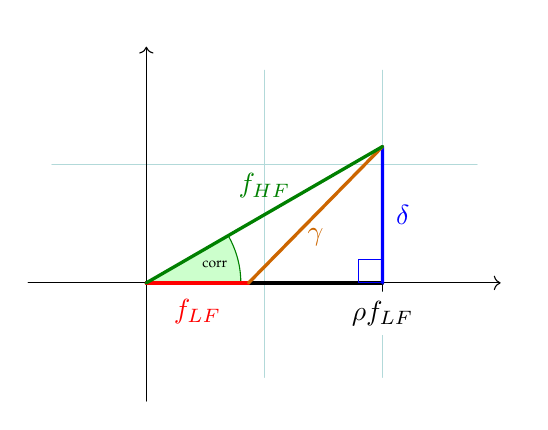
\begin{tikzpicture}[scale=3,cap=round]
  % Local definitions
  \def\costhirty{0.8660256}
 \coordinate (A) at (0.8, 0) {};\
 \coordinate (C) at (1, 0.2) {};
 \coordinate (0) at (1, 0) {};
  % Colors
  \colorlet{HF}{green!50!black}
  \colorlet{LF}{red}
  \colorlet{gamma}{orange!80!black}
  \colorlet{deltac}{blue}
  \colorlet{angle}{black}
  % Styles
  \tikzstyle{axes}=[]
  \tikzstyle{important line}=[very thick]
  \tikzstyle{information text}=[rounded corners,fill=red!10,inner sep=1ex]



  % The graphic
  \draw[style=help lines,step=0.5cm] (-0.4,-0.4) grid (1.4,0.9);
  %\draw (0,0) circle (1cm);
  \begin{scope}[style=axes]
    \draw[->] (-0.5,0) -- (1.5,0) node[right]{}; %{$x$};
    \draw[->] (0,-0.5) -- (0,1) node[above]{}; %{$y$};

%% Drawing 0.5 and 1
    %\foreach \x/\xtext in {-1, -.5/-\frac{1}{2}, 1}
      \draw[xshift=1 cm, angle] (0pt,1pt) -- (0pt,-1pt) node[below,fill=white]{$\rho f_{LF}$};
            %{$\xtext$};

%    \foreach \y/\ytext in {-1, -.5/-\frac{1}{2}, .5/\frac{1}{2}, 1}
%      \draw[yshift=\y cm] (1pt,0pt) -- (-1pt,0pt) node[left,fill=white]
%            {$\ytext$};
%% end drawing 0.5 and 1
  \end{scope}
  \filldraw[fill=green!20,draw=green!50!black] (0,0) -- (4mm,0pt) arc(0:30:4mm);
  \draw (15:3mm) node[angle] {\tiny corr};
  
  \draw[style=important line,angle]
    (0,0) -- (1,0);
  
  \draw[style=important line,LF]
    (0,0) -- node[below=2pt] {$f_{LF}$} (\costhirty/2,0);

  \draw[style=important line,deltac] (1,0) --
    node [right=1pt]
    {$\delta$} (intersection of 0,0--30:1cm and 1,0--1,1) coordinate (t);
    
  \draw[style=important line,gamma]
    (\costhirty/2,0) -- node[below=1pt] {$\gamma$} (t);
   \tkzMarkRightAngle[draw=blue,size=.1](A,0,C);
  
  \draw[style=important line,HF] (0,0) --node[above=2pt] {$f_{HF}$} (t) ;
\end{tikzpicture}
}
\end{column}
\begin{column}{0.45\linewidth}
\scriptsize
-- Additive formulation \cite{VFM}
\begin{equation*}
f_{HF}(x) = f_{LF}(x) + \gamma(x)
\label{eq:vfm}
\end{equation*}
-- Kennedy-O'Hagan \cite{KeO}
\begin{equation*}
\left\{
\begin{array}{ll}
&f_{HF}(x) = \rho f_{LF}(x) + \delta(x)\\
&f_{LF}(\cdot) \perp \delta(\cdot)
\end{array}
\right.
\label{eq:mfk}
\end{equation*}
\end{column}
\end{columns}
\normalsize
\only<1->{\begin{itemize}
      \item[--] The addition of the term $\rho$ makes the multi-fidelity learning more robust to poor correlation as well as differences in modelization.
      \end{itemize}}
\end{frame}

\begin{frame}[fragile]
  \frametitle{Multi-Fidelity co-Kriging -- Toy Problem}
  \begin{columns}
    \begin{column}{0.6\linewidth}
  	\begin{center}
    \fontsize{7pt}{7pt}\selectfont Animation: evolution of model for increasing signal correlations
    \[f_{HF}(x) = \rho f_{LF}(x) + \delta(x)\]
  	\animategraphics[loop,width=\linewidth]		{2}{Kriging/cos_corr_}{0}{10}
 	\end{center}
  	\end{column}
    \begin{column}{0.4\linewidth}
    Functions definition for \(\alpha \in [0, \pi/2]\):
    \begin{align*}
		& f_{HF}(x) = \cos(x) \\
		& f_{LF}(x) = \textcolor{orange!80!black}{2} \cos(x+\textcolor{orange!80!black}{\alpha})
	\end{align*}
    HF-LF correlation:
    \[\operatorname{corr} (f_{HF},f_{LF}) = cos(\alpha)\]
    \end{column}
  \end{columns}
  \small
  \begin{itemize}
      \item[--]The use of mutli-fidelity information sources reduces the amount of information to be retrieved by the highest fidelities.
  \end{itemize}
\end{frame}

\begin{frame}
	\frametitle{Multi-Fidelity co-Kriging -- Contributions}
    \begin{columns}
    \begin{column}{0.4\linewidth}
    \begin{center}
    
    \end{center}
    Recursive formulation \cite{legratiet:tel-00866770}:
    \begin{align*}
&\mu_{k} = \rho_{k-1}\;\mu_{k-1} + \mu_{\delta_k} \\
&\sigma^2_{k} = \rho_{k-1}^2\;\sigma^2_{k-1}+\sigma^2_{\delta_k} \label{eq:rec_sigma_l}
\end{align*}
-- Nested DOEs:\[X_{HF}=X_l \subseteq X_{l-1} \ldots  \subseteq X_0=X_{LF} \]

    \end{column}
    \begin{column}{0.6\linewidth}
    \scriptsize
    \begin{itemize}
    \item[$\ast$] MFK \cite{vauclin2015,MFK_OpenMDAO}
    \item[$\ast$] MFKPLS - MFKPLSK (high dimension)
    \item[$\ast$] Analytical derivatives w.r.t design variables
    \item[$\ast$] Noise Estimation
    \item[$\ast$] Regression/ Re-interpolation
    \item[$\ast$] multi-fidelity data pre-processing
    \end{itemize}
    \normalsize
    \end{column}
    \end{columns}
    \begin{columns}
    \begin{column}{0.75\linewidth}
    \small
    Open source Python library: Surrogate Modeling Toolbox (SMT)
    
    \url{https://github.com/SMTOrg/smt}
    \end{column}
    \begin{column}{0.25\linewidth}
    \includegraphics[width=0.8\linewidth]{images/logosmt}
    \end{column}
    \end{columns}
\end{frame}

\section{Bayesian Optimization}
\label{sec:partie2}
\begin{frame}[fragile]
  \frametitle{Bayesian Optimization}
  	\begin{columns}
  	\begin{column}{0.45\linewidth}
    \begin{itemize}
    \item[\scriptsize$\blacksquare$] \only<1->{\textbf{Gradient-based}: minimize the objective gradient norm.}
    \item[\scriptsize$\blacksquare$] \only<1->{\textbf{Bayesian (gradient-free)}: minimize the expected deviation from the extremum of the studied function.}
    \end{itemize}
      
      \end{column}
      \begin{column}{0.55\linewidth}
      \begin{center}
        \includegraphics[width=6cm]{Bayesian/vartrue}
        %\captionof{figure}{Multi-Fo co-Kriging characteristic length evolution w.r.t correlation}
      \end{center}
      \end{column}
	\end{columns}
    \only<2->{
    \begin{itemize}
    \item[--] Prediction and uncertainty of the model are used in sequential strategies to balance Exploration/Exploitation
    \item[--] Bayesian optimization is a global optimization.
    \end{itemize}
    }
\end{frame}


\subsection{Efficient Global Optimizaton: EGO}    
\begin{frame}
  \frametitle{Bayesian Optimization -- EGO}
  \begin{columns}
  	\begin{column}{0.45\linewidth}
    \small
    Efficient Global Optimization \cite{Jones:1998:EGO:596070.596218} 
    
    \vspace{0.3cm}
    
      -- EI criterion \cite{Mockus1975}:\[ E[I(x)] = E[\max(f_{min}-Y, 0)]\]
      \end{column}
      \begin{column}{0.55\linewidth}
      \begin{center}
        \includegraphics[width=6cm]{Bayesian/EImax}
        %\captionof{figure}{Multi-Fo co-Kriging characteristic length evolution w.r.t correlation}
      \end{center}
      \end{column}
	\end{columns}
    \normalsize
   \begin{itemize}
      \item[--] EI expresses a certain balance between Exploitation and Exploration based on the mean and variance of the Kriging model.
      \end{itemize}
   
\end{frame}

\subsection{Multi-Fidelity Efficient Global Optimizaton: MFEGO}
\begin{frame}[fragile]
	\frametitle{Bayesian Optimization -- MFEGO}
    \only<1->{MFEGO:
    \begin{itemize}
    \item most promising point: EI criterion\[\textcolor{orange!80!blue}{x^*} = \argmax_{x} \left(E[I(x)]\right)\]
    \item choice of levels of enrichment: trade-off information gain/cost \[\textcolor{orange!80!blue}{k^*} = \argmax_{k \in (0,\ldots,l)} \quad \frac{\sigma_{red}^{2}(k,\textcolor{orange!80!blue}{x^*})}{f(c_{k})}\]
    \end{itemize}
    
    }
    
    \only<2->{
    \small
    \begin{itemize}
    \item[$\Rightarrow$] By using low-fidelity to reduce the uncertainty we reduce the Exploration contribution to the EI criterion
    \item[$\Rightarrow$] High-fidelity is used for Exploitation and model enhancement
    \end{itemize}}
\end{frame}

\begin{frame}[fragile]
  \frametitle{MFEGO Optimization -- Toy Problem}
  \begin{columns}
  
  \begin{column}{0.65\linewidth}
  \begin{center}
  	\animategraphics[loop, controls,width=\linewidth]		{1}{Bayesian/foo}{1}{10}
 	\end{center}
  \end{column}
  \begin{column}{0.35\linewidth}
  \begin{center}
  \includegraphics[width=\textwidth]{Bayesian/testcase}
  \end{center}
  \tiny
  \begin{align*}
f_{HF}(x) =&\;(6  x -2)^2 \times \sin(2(6 x - 2))\\
f_{LF}(x) =&\;0.5 f_{HF} + 10 (x-0.5) - 5
\end{align*}
Cost ratio: 1/1000
 \begin{tabular} {  l  c  c  c }
 \hline
 & HF & LF & Cost \\
 \hline
 \hline
 MFEGO  & \textcolor{green!40!black}{3}+2  & \textcolor{green!40!black}{6}+9 & \textcolor{blue}{5.015}\\
  EGO  & \textcolor{green!40!black}{4}+11  & - & \textcolor{red}{15}\\
\hline
\end{tabular} 
  \captionof{table}{\fontsize{7pt}{7pt}\selectfont Toy problem optimization summary}
  \end{column}
  \end{columns}
\end{frame}
    


\section{Application to Airfoil Shape Optimization}
\label{sec:partie2}
\begin{frame}[fragile]
  \frametitle{Airfoil shape optimization -- Parametrization}
  \begin{columns}
  \begin{column}{0.6\textwidth}
     \begin{tikzpicture}
  \node(HF) at (0,0) {\includegraphics[width=0.8\textwidth]{images/thickness_modes}};
  \node(SM) at (0,-2) {\includegraphics[width=\textwidth]{images/camber_modes}};
  \end{tikzpicture}
  \captionof{figure}{First thickness (above) and camber (below) modes \cite{Jichao}}
  \end{column}
  \begin{column}{0.4\linewidth}
  \scriptsize
  Parametrization \cite{Jichao}:
  Mode decomposition of an airfoil database.
  
  Up to 14 modes available (7 camber + 7 thickness modes).
  
  \begin{itemize}
  \item[$\ast$] HF: RANS solver (ADflow)
  \item[$\ast$] LF: Xfoil \cite{drela1989xfoil}
  \end{itemize}
  Cost ratio: 1/200
  
  Reference: SNOPT \cite{gill2005snopt}
  \end{column}
  \end{columns}
\end{frame}




\begin{frame}
  \frametitle{Airfoil shape -- Unconstrained optimization}
  \begin{center}
  \only<1>{
   \begin{tikzpicture}
  \node(HF) at (0,0) {\includegraphics[width=0.55\textwidth]{Results/run_full_3}};
  \node(DOE) at (0.5\textwidth,0) {\includegraphics[width=0.55\textwidth]{Results/same}};
  \end{tikzpicture}
  }
   \only<2>{
   \begin{tikzpicture}
  \node(HF) at (0,0) {\includegraphics[width=0.55\textwidth]{Results/run_full_3}};
  \node(DOE) at (0.5\textwidth,0) {\includegraphics[width=0.55\textwidth]{Results/best_run_same}};
  \end{tikzpicture}
  }
  \only<3>{
 \begin{tabular} {  l  c  c  c  c }
 \hline
 & HF & LF & Cost & Obj \\
 \hline
 \hline
 EGO & \textcolor{green!40!black}{40} + 30 & - &  \textcolor{red}{70} & \textcolor{red}{104.9} \\
 MFEGO  & \textcolor{green!40!black}{16} + 8  & \textcolor{green!40!black}{744} + 437 & \textcolor{blue}{29.89} & \textcolor{blue}{110.5} \\
 SNOPT  & \textcolor{green!40!black}{21} & - & 21 & 110.7 \\
\hline
\end{tabular} 
  \captionof{table}{Comparison of EGO and MFEGO for unconstrained optimization}
  
  \vspace{3em}
  }
  \end{center}
  \begin{itemize}
  \item L/D maximization
  \item \textcolor{blue}{15} design variables (7 camber + 7 thickness modes + AoA)
  \end{itemize}
\end{frame}


\begin{frame}
  \frametitle{Airfoil shape -- Constrained optimization}
  \begin{center}
  \only<1>{
    \begin{tikzpicture}
  \node(HF) at (0,0) {\includegraphics[width=0.55\textwidth]{Results/2constrained}};
  \node(DOE) at (0.5\textwidth,0) {\includegraphics[width=0.55\textwidth]{Results/2Constraints_scaled}};
  \end{tikzpicture}}
  \only<2>{
  \begin{center}
  \scriptsize
 \begin{tabular}{lcccccc}
\hline
& HF & LF & Cost & Obj & Feasible & RMSCV\\
\hline
\hline
EGO  & \textcolor{green!40!black}{40} + 60 & - & \textcolor{red}{100} & \textcolor{red}{89.188} & Yes & \textcolor{red}{8.8e-2} \\
MFEGO & \textcolor{green!40!black}{24} + 18 & \textcolor{green!40!black}{964} + 63 & \textcolor{blue}{47.135} & \textcolor{blue}{84.67} & Yes & \textcolor{blue}{4.9e-3} \\
SNOPT & \textcolor{green!40!black}{73} & - & 73 & 84.68 & Yes & - \\
\hline
\end{tabular} 
  \captionof{table}{Comparison of EGO and MFEGO for constrained optimization}
  \end{center}
  \normalsize
  \(RMSCV = \sqrt[]{\frac{1}{N} \sum_{j=1}^N \left(val_j-target\right)^2}\)
  \vspace{1em}
  }
  \end{center}
  -- Use of SEGOMOE framework \cite{bartoli2016improvement}
  \begin{itemize}
  \item $C_d$ minimization
  \item $C_l$, $C_m$ equality constraints
  \item \textcolor{blue}{15} design variables (7 camber + 7 thickness modes + AoA)
  \end{itemize}
\end{frame}

\section{Conclusion}
\begin{frame}
  \frametitle{Conclusion \& Perspectives}
  This project has shown it is possible to use multi-fidelity information sources to:
  \small
  \begin{itemize}
  \item enhance surrogate models $\rightarrow$ \textcolor{green!10!orange!90!}{MFK integration in SMT},
  \item alleviate dimensionality curse $\rightarrow$ \textcolor{green!10!orange!90!}{MFKPLS -- MFKPLSK},
  \item reduce global search cost (global optimizations) $\rightarrow$ \textcolor{green!10!orange!90!}{MFEGO},
  \item find better results with lesser cost compared to EGO (and occasionally SNOPT) for multiple constrained and unconstrained problems $\rightarrow$ \textcolor{green!10!orange!90!}{SEGOMOE framework extension}.
  \end{itemize}
  -- In progress: \textcolor{green!10!orange!90!}{AIAA Aviation 2019 Conference abstract submission}, \textcolor{green!10!orange!90!}{aerostructural optimization test case.}
  
  \vspace{0.3cm}
  \normalsize
  Work can be done to improve the approach:
  \scriptsize
  \begin{itemize}
  \item hybrid models (a different model adapted to each level of fidelity)
  \item multi-fidelity mixture of experts,
  \item ...
  \end{itemize}
\end{frame}

\begin{frame}
  \frametitle{Questions}
  \begin{tikzpicture}[overlay]
  \node [anchor=center] at (9,2) {\includegraphics[width=0.2\linewidth]{images/fondation}};
  \end{tikzpicture}
  \begin{center}
    Thank you for your attention!

    Do you have any questions?
  \end{center}
\end{frame}

\newcounter{lastframe}
\setcounter{lastframe}{\insertframenumber}

\begin{frame}[allowframebreaks]{References}
\bibliographystyle{authoryear-fr}
\bibliography{references}
 \end{frame}
\setcounter{framenumber}{\thelastframe}
\end{document}
